\documentclass{beamer}
%\documentclass[handout]{beamer}

\usepackage{ensislides}
\usepackage[utf8]{inputenc}
\usepackage[french]{babel}

\title[Fully Homomorphic Encryption Scheme]{Analyzing Security-Cost Trade-off for a\\Fully Homomorphic Encryption Scheme}

%\subtitle{Un exemple} % (optional)

%\author{Matthieu Moy}
\author{Amrit Kumar \\ Kais Chaabouni \\}
\date{\today}
% - Use the \inst{?} command only if the authors have different
%   affiliation.

\institute{Ensimag}
%\date{2012-2013}

\begin{document}

\begin{frame}
  \titlepage
\end{frame}

\section{Introduction}

\begin{frame}\frametitle{Introduction}
  \begin{itemize}
  \item What is FHE, what properties it provides?\\
    
    \begin{itemize}
      \pause
    \item Partially HE: ex RSA: $c_1c_2=(m_1m_2)^e \ \textrm {mod}\ N$
      \pause
    \item $\mathcal{E}(x_1).\mathcal{E}(x_2)=\mathcal{E}(x_1.x_2)$ , $\mathcal{E}(x_1)+\mathcal{E}(x_2)=\mathcal{E}(x_1+x_2)$   
      
    \end{itemize}
    \pause
  \item Gentry's scheme and other schemes.  
    
    \begin{itemize}
      \pause
    \item ``Somewhat'' HE. \\ 
      \pause
      $r(c_1+c_2) < r(c_1)+r(c_2)$ , $r(c_1.c_2) < r(c_1).r(c_2)$
      \pause
    \item ``Bootstrapping'' \\ 
      \pause
      ``dirty'' cipher-text $\rightarrow$ ``clean'' cipher-text
      
    \end{itemize}
    \pause
  \item Implementations, Cost, Security. \\
    
    \begin{itemize}
      \pause
    \item \texttt{Min}, \texttt{Max} of $(a,b)$ on plain-text:
       \newline \phantom{x}\hspace{3ex}  \texttt{Max}= $a > b$? $a$ : $b$ 
       \newline \phantom{x}\hspace{3ex}   \texttt{Min}= $a \leq b$? $a$ : $b$ 
      \pause
     \item \texttt{Min}, \texttt{Max} of $(a,b)$ on cipher-text ?

    \end{itemize}
  \end{itemize}
\end{frame}

\section{Theoretical Analysis}

\subsection{SV Scheme: cost-security of crypto-system}

\begin{frame} \frametitle{SV Scheme: cost-security of crypto-system}


    \begin{block}{\texttt{KeyGen}}

    $F(x)=X^{2^n}+1$
    \newline Do until p is prime\{ $S(x) \leftarrow_{R}B_{\infty , N}(\eta/2)$\;
    \newline \phantom{x}\hspace{3ex} $G(x)=1+2.S(x)$ 
    \newline \phantom{x}\hspace{3ex} $p= \mathrm{\textbf{resultant}}(G(x),F(x))$ \}
    \newline $D(x)=\mathrm{\textbf{gcd}}(G(x),F(x))$ over $\mathbb{F}_p[x]$
    \newline $\alpha$ $\leftarrow$ unique root of $D(x) \in \mathbb{F}_p $
    \newline apply \texttt{xgcd} algorithm over $\mathbb{Q}[x]$ to obtain $Z(x).G(x)=p$ mod $F(x)$
    \newline $B=z_0$ mod $2p$
    $pk = (p, \alpha)$ and $sk = (p , B)$
\end{block}
\end{frame}

\begin{frame} \frametitle{Continued}
\begin{block}{Encrypt/Decrypt(pk,sk)}
 $R(x) \leftarrow_{R}B_{\infty , N}(\mu/2)$
    \; $C(x)=m+2\cdot R(x)$ 
    \newline \phantom{x}\hspace{3ex} return  $c=C(\alpha)$ mod $p$;
    \newline \texttt{Decrypt}($c, sk$):
    \newline \phantom{x}\hspace{3ex} $m = (c - \lfloor c \cdot B/p \rceil )$ mod $2$;
\end{block}

\begin{block}{Operations}
    \texttt{Add}($c_1$, $c_2$, $pk$):
    \newline \phantom{x}\hspace{3ex} $c_3=c_1+c_2$ mod $p$; 
    \newline \texttt{Mult}($c_1$, $c_2$, $pk$):
    \newline \phantom{x}\hspace{3ex}  $c_3=c_1.c_2$ mod $p$; 
\end{block}
\begin{itemize}
  \item security : $\frac{N}{\epsilon}$ with $2 ^ \epsilon = \frac{\eta}{2\cdot \mu \sqrt{N}} $
  \item depth :  $d \cdot \mathrm{log}(2) \leq  \mathrm{log}\left( \mathrm{log}\left(\frac{\eta}{2\cdot \sqrt{N}}\right) \right) - \mathrm{log}\left(\mathrm{log}\left( N\mu\right)\right)$
  \end{itemize}
\end{frame}

\subsection{Programs on ciphertexts}


\begin{frame} \frametitle{ Straight-line vs Non-Straight-line}
  \begin{itemize}
  \item Straight line $\rightarrow$ translates directly
  \item Non-Straight line $\rightarrow$ circuit transformation(\textcolor{orange}{Always ?})
  \end{itemize}

\begin{columns}
\begin{column}[c]{9cm}
\begin{exampleblock}{Non-secret branching : XOR}
\texttt{a[0, $\ldots,$ n-1], res=0, i=0;}
\newline \phantom{x} \texttt{do\{ }
\newline \phantom{x} \hspace{9ex} \texttt{res=res$\oplus$a[i];}
\newline \phantom{x} \hspace{9ex} \texttt{i++;} 
\newline   \phantom{x} \} \texttt{while(i < n);} \phantom{x} \hspace{9ex}\texttt{// i, n} \textcolor{orange}{not secret}
\end{exampleblock}
\end{column}
\begin{column}[c]{2cm}

 %YOUR SECOND COLUMN HERE
\end{column}
\end{columns} 
\begin{alertblock}{Secret branching}
\texttt{if(a' > b') instn\_1; else instn\_2;}
\newline   \phantom{x}  \hspace{8ex} $\Rightarrow$ \texttt{test(a'> b')$\wedge$} \texttt{instn\_1 +} $\neg$\texttt{test(a'> b')$\wedge$ instn\_2 }
\newline \textcolor{orange}{Cost} = linear
\end{alertblock}
\end{frame}

\begin{frame} 
 \frametitle{Conditional stopping }
\restylealgo{algoruled}
\linesnumbered 
\begin{columns}
\begin{column}[c]{8cm}

\begin{block}{\texttt{test(a'>b')}}
\begin{algorithm}[H]

\SetVline
 $aIsGreater \leftarrow 0$\;
 $bitEqual \leftarrow 1$\;
	
 \For{$i\leftarrow 0 $ \KwTo $n-1$}{
						
     $aIsGreater \leftarrow aIsGreater \vee (\neg(b_i')\wedge a_i'\wedge bitEqual$) \;
     $bitEqual \leftarrow bitEqual\wedge((a_i'\wedge b_i')\vee(\neg(a_i)'\wedge\neg(b_i')))$\;	       	
 }

\caption{test(a'$>$b')\label{Code:algo}}
\end{algorithm}
\end{block}
\end{column}
\begin{column}[c]{3cm}
 $\Rightarrow$ \textcolor{orange}{Max/Min ?}
\end{column}
\end{columns} 

\begin{columns}
\begin{column}[c]{8cm}
\begin{block}{Min-Max}
 $Max_i \leftarrow (aIsGreater \wedge a_i') \vee (b_i'\wedge \neg(aIsGreater))$ \;
 $Min_i \leftarrow  (a_i' \wedge \neg(aIsGreater) ) \vee (aIsGreater \wedge b_i')$ \;
\end{block}
\end{column}
\begin{column}[c]{2cm}
$\Rightarrow$ \textcolor{orange}{spectrum of funcs}
\end{column}
\end{columns}
\end{frame}

\subsubsection{Tested Operations}
\begin{frame} \frametitle{Tested Operations}
  \begin{itemize}
  \item XOR(of $n$ bits), Majority of $n$-bits, Sum of integers($<32$ bits)
   \item Matrix product
  \item Sorting
   \begin{itemize}
   \item Insertion sort : $n(n-1)/2$
   \item Bitonic sort : $n\mathrm{log}(n)(\mathrm{log}(n)+1)/4$ comparators
    \item Odd-Even sort : $n(\mathrm{log}^{2}(n)-1)/2 + 1 $ comparator
   \end{itemize}
\end{itemize}
sorting $\rightarrow$ \textcolor{orange}{Sorting network}
\begin{columns}
\begin{column}[c]{3cm}
\begin{figure}%on ouvre l'environnement figure
\vspace{-3ex}
\centering
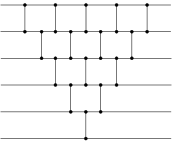
\includegraphics[width=3cm, height=3cm]{network.png} 
\caption{Insertion Sort Network } 
 %l'étiquette pour faire référence à cette image
\end{figure}
\end{column}
\begin{column}[c]{3cm}
\begin{figure}
\vspace{-3ex}
\centering
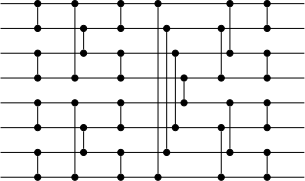
\includegraphics[width=3cm, height=3cm]{networkBitonic.png} 
\caption{Bitonic Sort Network } 
 %l'étiquette pour faire référence à cette image
\end{figure}
\end{column}
\begin{column}[c]{3cm}
\begin{figure}
\vspace{-5ex}
\centering
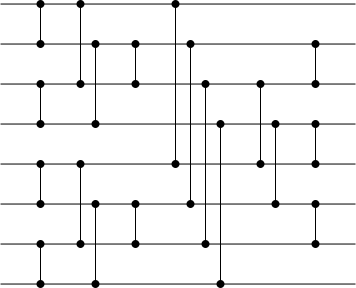
\includegraphics[width=3cm, height=3cm]{networkOdddEven.png} 
\caption{Odd-Even Merge Sort Network } 
 %l'étiquette pour faire référence à cette image
\end{figure}
\end{column}
\end{columns}

\end{frame}



\section[Experimental Analysis]{Experimental Analysis}

\subsection{Security-Cost}

\begin{frame} \frametitle{titre3.1}
  \begin{itemize}
  \item cost of keyGen
  \item Cost depending on security parameters N, eta, mu of crypto system / program
  \item \warning{depth too little: wrong decryption}
  \item explication
  \end{itemize}
\end{frame}

\subsection{Implementations cost}

\begin{frame} \frametitle{Results}

\begin{columns}
\begin{column}[c]{3cm}
\begin{figure}%on ouvre l'environnement figure
\vspace{-3ex}
\centering
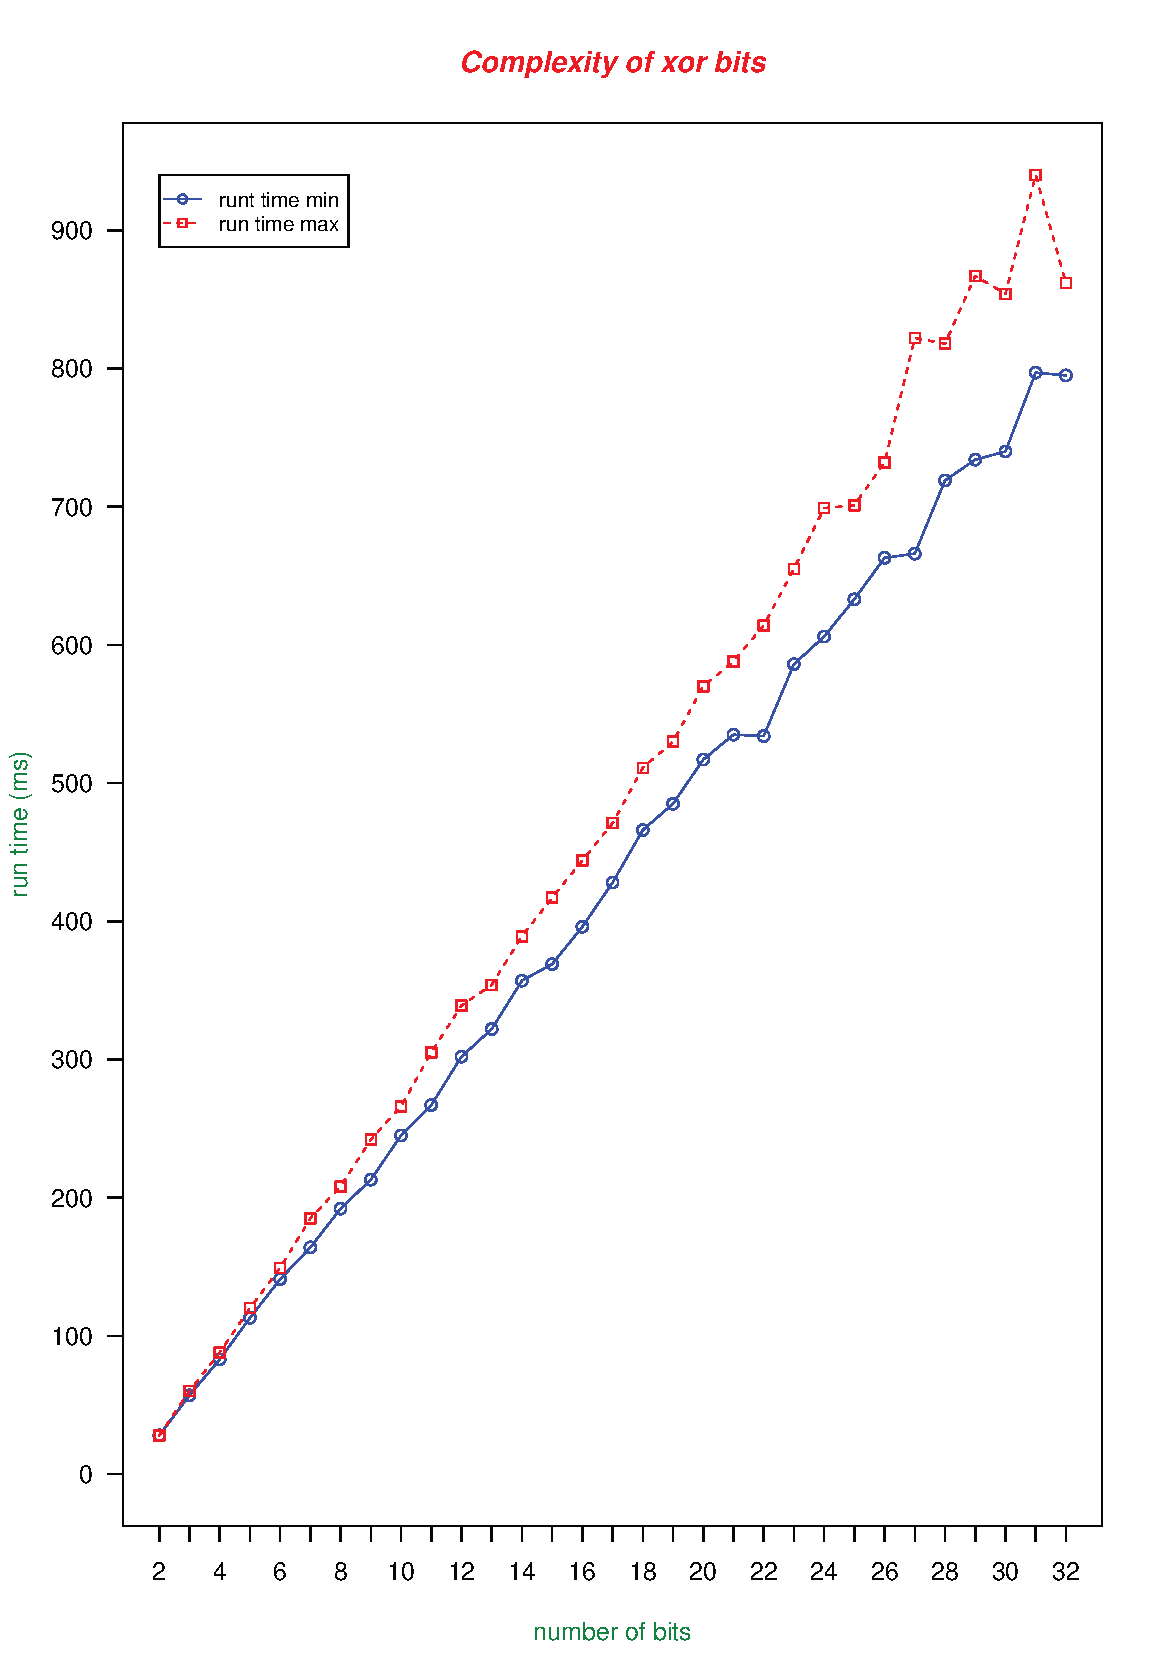
\includegraphics[width=5cm, height=5cm]{f4.pdf} 
\caption{XOR of $n$ bits} 
 %l'étiquette pour faire référence à cette image
\end{figure}
\end{column}
\begin{column}[c]{5cm}
\begin{figure}
\vspace{-2cm}
\centering
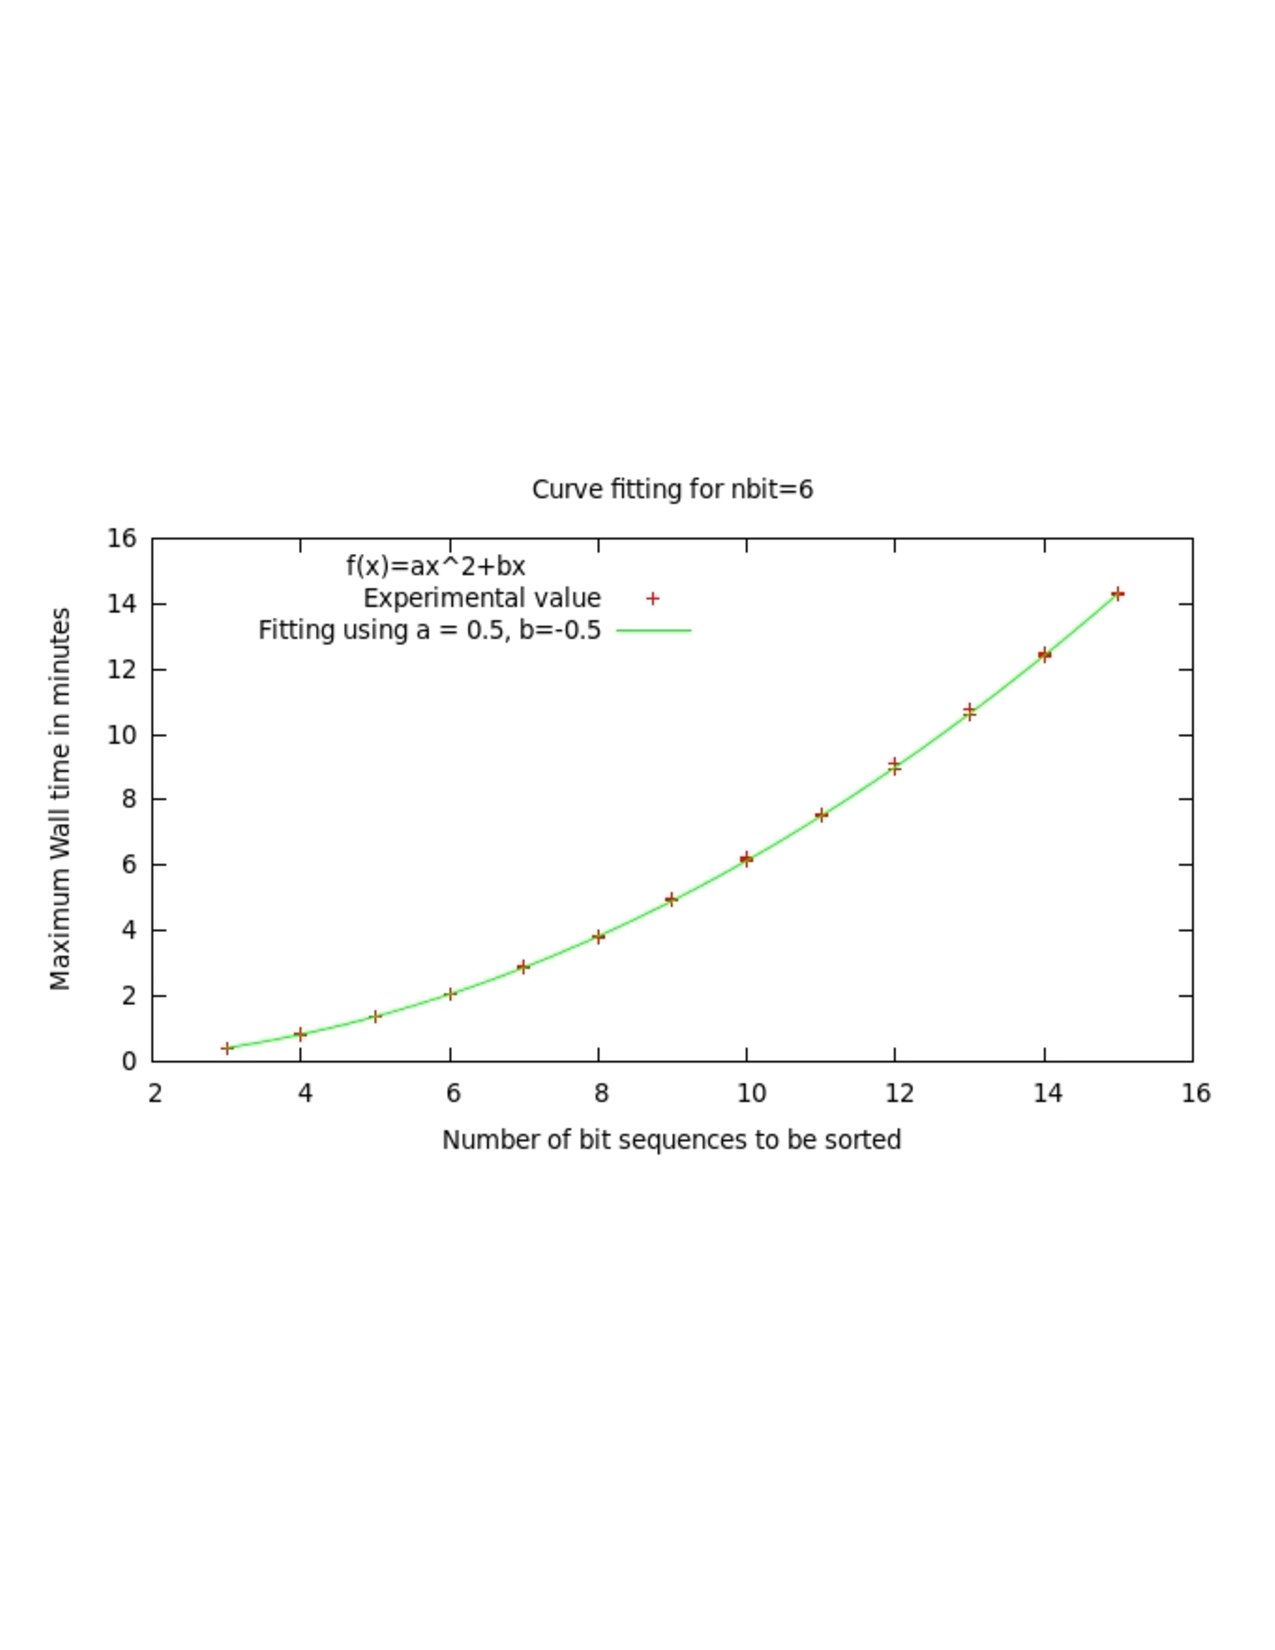
\includegraphics[width=6cm, height=8cm]{fsort1.pdf} 
\caption{Insertion sort nbit=6} 
 %l'étiquette pour faire référence à cette image
\end{figure}
\end{column}
\end{columns}

\end{frame}

\begin{frame} \frametitle{Results}
 \begin{columns}
\begin{column}[c]{3cm}
\begin{figure}%on ouvre l'environnement figure
\vspace{-3ex}
\centering
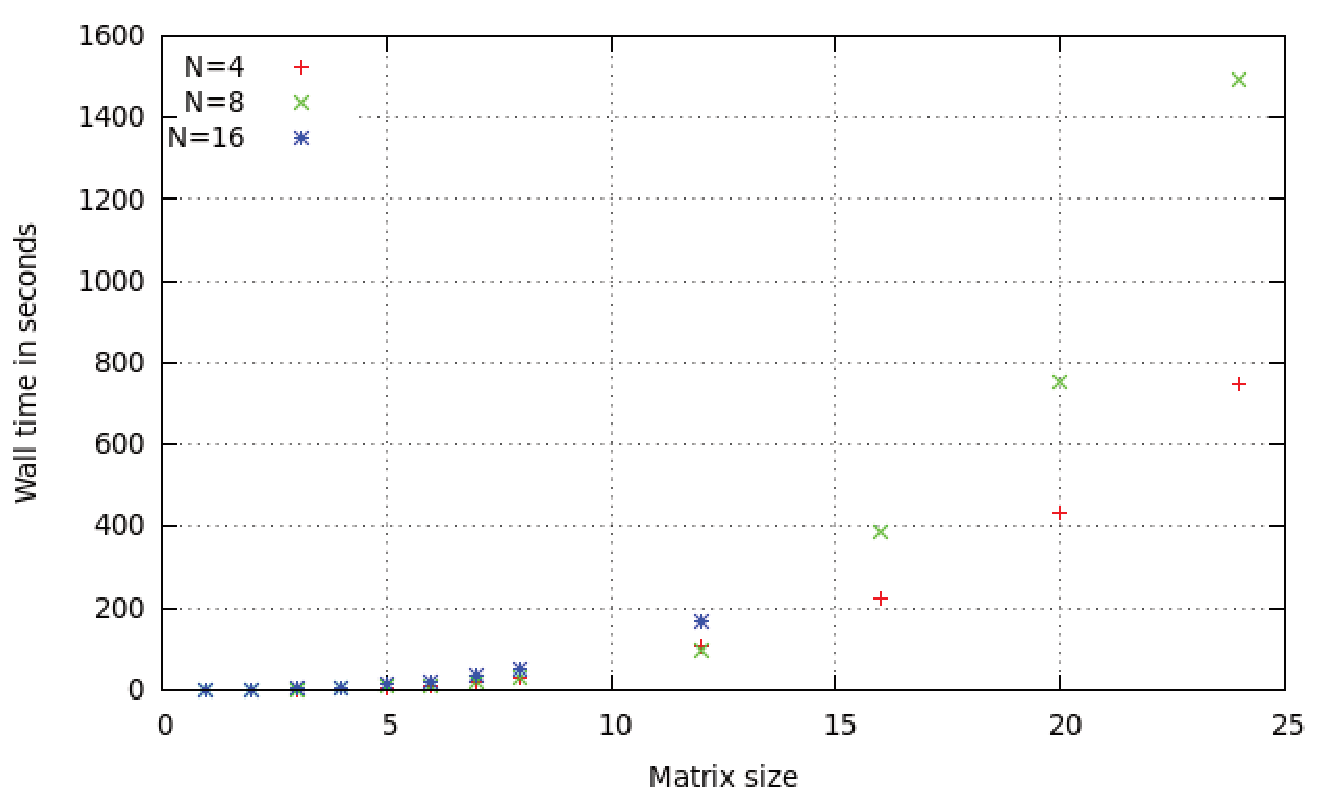
\includegraphics[width=5cm, height=5cm]{f9.pdf} 
\caption{Matrix product} 
 %l'étiquette pour faire référence à cette image
\end{figure}
\end{column}
\begin{column}[c]{4cm}
\begin{table}
\caption{Wall time for Odd-Even Merge Sort}
\resizebox{5cm}{!}{
\begin{tabular}{|l|l|l||}
  \hline
  (Number of sequences,  & Maximum time (in ms) & Minimum time (in ms) \\
  Number of bits) &  &    \\
  \hline
  (4, 4) & 28363 & 27321  \\
  (8, 4)  & 158674 & 120868 \\
  (16,4) & 459895  & 340981  \\
  (32,4) & 1043093 &  1041674 \\
  (4,6) & 41350 & 41204 \\
  (8,6) & 158272  &156721 \\
  (16,6) & 543735 & 520719 \\
  (32,6) & 1638711 & 1594432 \\
\hline
\end{tabular}
\label{OddEvensort1}
}
\end{table}
\end{column}
\end{columns}
\end{frame}

\section[Conclusion]{Conclusion}

\begin{frame}
  \frametitle{Conclusion}
  \begin{itemize}
  \item Transformation on programs (no jump nor branching)

  \item Cost of program

  \item Security and Cost

  \item Quality cryptosystem
  \end{itemize}
\end{frame}

\end{document}


%%% Local Variables: 
%%% mode: latex
%%% TeX-master: t
%%% End: 
